\documentclass[tikz,border=5pt]{standalone}
\usepackage{amssymb,amsmath}
\newcommand{\C}{\mathbb{C}}
\newcommand{\CP}{\mathbb{CP}}
\begin{document}
%========================================================
% FIGURE 2: X = C / Lambda (complex torus)
%========================================================
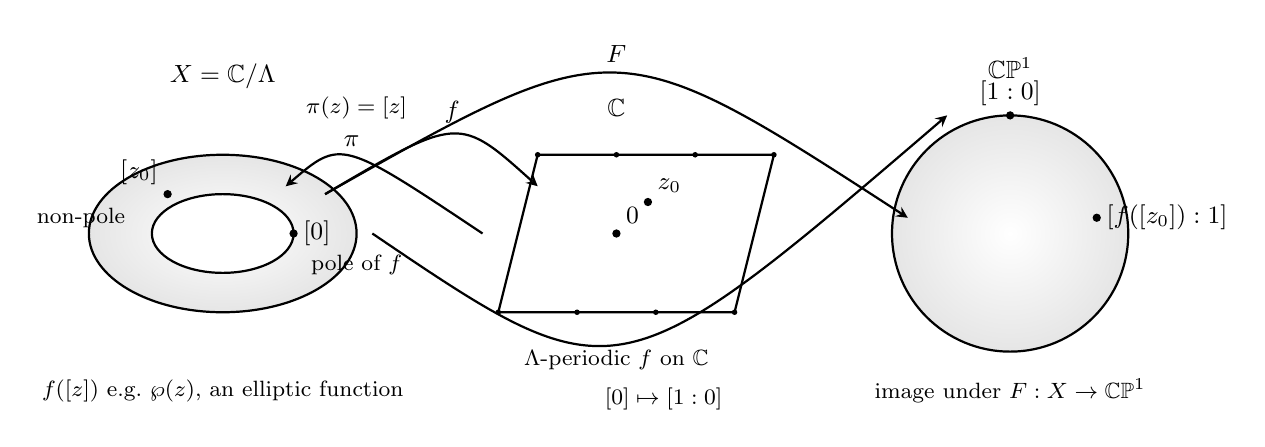
\begin{tikzpicture}[font=\small,>=stealth]
	
	%----------------------------
	% Left: Domain X = C / Lambda (torus)
	%----------------------------
	\begin{scope}[shift={(-5,0)}]
		% A simple torus shape (donut)
		% outer ellipse
		\shade[inner color=white, outer color=gray!20, draw=black, thick]
		(0,0) ellipse (1.7 and 1.0);
		% inner ellipse (hole)
		\fill[white]
		(0,0) ellipse (0.9 and 0.5);
		\draw[black,thick]
		(0,0) ellipse (0.9 and 0.5);
		
		\node at (0,2.0) {$X=\mathbb{C}/\Lambda$};
		
		% point [0] (pole of elliptic function)
		\fill (0.9,0) circle (1.5pt);
		\node[right] at (0.9,0) {$[0]$};
		\node at (1.7,-0.4) {\footnotesize pole of $f$};
		
		% non-pole point [z0]
		\fill (-0.7,0.5) circle (1.5pt);
		\node[above left] at (-0.7,0.5) {$[z_0]$};
		\node at (-1.8,0.2) {\footnotesize non-pole};
		
		% explanation
		\node at (0,-2.0) {\footnotesize $f([z])$ e.g.\ $\wp(z)$, an elliptic function};
	\end{scope}
	
	%----------------------------
	% Middle: Complex plane C with lattice
	%----------------------------
	\begin{scope}
		% fundamental parallelogram for Lambda
		\draw[thick] (-1.5,-1) -- (1.5,-1) -- (2,1) -- (-1,1) -- cycle;
		\node at (0,1.6) {$\mathbb{C}$};
		
		% indicate lattice points (roughly)
		\foreach \x/\y in {-1.5/-1, -0.5/-1, 0.5/-1, 1.5/-1,
			-1/1, 0/1, 1/1, 2/1}
		\fill (\x,\y) circle (1pt);
		
		% origin 0 (pole in cover)
		\fill (0,0) circle (1.5pt) node[above right] {$0$};
		
		% point z0
		\fill (0.4,0.4) circle (1.5pt) node[above right] {$z_0$};
		
		% note lattice
		\node at (0,-1.6) {\footnotesize $\Lambda$-periodic $f$ on $\C$};
	\end{scope}
	
	%----------------------------
	% Right: Target CP^1
	%----------------------------
	\begin{scope}[shift={(5,0)}]
		% Sphere for CP^1
		\shade[inner color=white, outer color=gray!20, draw=black, thick]
		(0,0) circle (1.5);
		\node at (0,2.1) {$\mathbb{CP}^1$};
		
		% north pole = [1:0]
		\fill (0,1.5) circle (1.5pt);
		\node[above] at (0,1.5) {$[1:0]$};
		
		% equator point = [f([z0]):1]
		\fill (1.1,0.2) circle (1.5pt);
		\node[right] at (1.1,0.2) {$[f([z_0]):1]$};
		
		\node at (0,-2.0) {\footnotesize image under $F:X\to\CP^1$};
	\end{scope}
	
	%----------------------------
	% Arrows: f, F, quotient pi
	%----------------------------
	
	% arrow pi: C -> X (quotient)
	\draw[->,thick]
	(-1.7,0.0) .. controls (-3.5,1.2) .. (-4.2,0.6)
	node[midway,above] {$\pi$};
	\node at (-3.3,1.6) {\footnotesize $\pi(z)=[z]$};
	
	% arrow f: X -> C (from [z0])
	\draw[->,thick]
	(-3.7,0.5) .. controls (-2,1.5) .. (-1.0,0.6)
	node[midway,above] {$f$};
	
	% arrow F: X -> CP^1 (from [z0])
	\draw[->,thick]
	(-3.7,0.5) .. controls (0,2.6) .. (3.7,0.2)
	node[midway,above] {$F$};
	
	% image of [0] under F: [0] -> [1:0]
	\draw[->,thick]
	(-3.1,0.0) .. controls (0,-2.1) .. (4.2,1.5);
	\node at (0.6,-2.1) {\footnotesize $[0]\mapsto[1:0]$};
	
\end{tikzpicture}	
\end{document}